%# -*- coding: utf-8-unix -*-
%%==================================================
\chapter{相对论基础}

本讲义的授课主题,是\gw\DA,共分为两部分,\emph{\gw}与\emph{\DA}。
如果脱离了\gw 的物理图景,而直接空谈\DA,未免空中楼阁。
而在另一方面,引力波又是Einstein广义相对论的直接理论预言,因此,引力波的理论描述,无法跳脱广义相对论的框架。

\begin{figure}[htp]
\centering
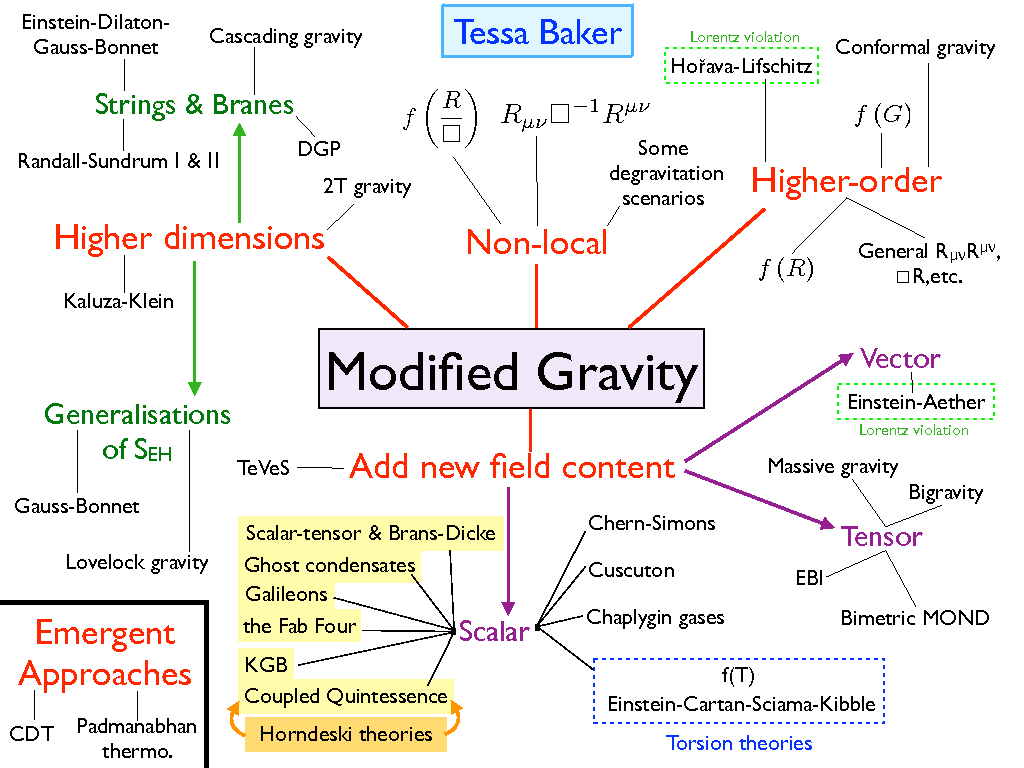
\includegraphics[width=0.7\textwidth]{ModifiedGravity.png}
\bicaption{修改引力理论}
  {Theories of modified gravity. Credit: http://www.cgc-yzu.cn/Upload/research/MG-20240317524.png}
\label{fig:ModGrav}
\end{figure}

从Einstein至今,引力理论已经有了长足的发展,如图\ref{fig:ModGrav}所示,仅基于\GR 基础上发展起来的修改引力理论就已不计其数。
由于和量子力学原理的深刻矛盾,有理由认为Einstein决定论性的的\GR 在某个地方一定背离了引力的物理本质。
然而,时至今日,Einstein昔日基于\GR 所作出的诸多预言,一一被实验所验证;所有可靠的实验检验下,\GR 均可以给出解释——而它通常是最简洁的那个理论。
因此,即使将来的实验证明了\GR 与引力的物理本质之间的偏离,对\GR 的理解依然有着重要的意义。

\section{相对性原理(Principle of relativity)}

\subsection{Galilean相对论}
虽然在20世纪,相对论一次专指Einstein的理论,但是相对性原理(Principle of relativity)的思想在Newtonian力学中就有体现:两个服从Newtonian力学的、相对均匀运动的惯性参考系,无法通过在内部展开的力学实验进行区分。
这一思想一般认为是Galileo在《关于Ptolemaic和 Copernican两大世界体系的对话》中首先提出的\cite{Fang2012blog}:
\begin{myprop}{}{}
把你和一些朋友关在一条大船的甲板下的主舱里,让你们带着几支苍蝇、蝴蝶和其他小飞虫,舱内放一支大碗,其中有几条鱼,然后,挂上一个水瓶,让水一滴一滴地滴到下面的一个宽口罐里。船停着不动时,你留神观察,小虫都以等速向舱内各方向飞行,鱼向各方向随便游动,水滴滴进下面的罐中。你把任何东西扔给你的朋友时,只要距离相等,向这一方向也不比向另一方向更多用力。你的双脚齐跳,无论向哪个方向跳过的距离都相等。当你仔细观察这些事情之后,再使船以任何速度前进,只要运动是均匀的,也不忽左忽右地摆动,你将发现,所有上述现象都没有丝毫变化,你无法从任何一个现象来确定,船是在运动还是在停着不动。即使船运动得相当快,在跳跃时,你也将和以前一样,你跳向船尾也不会比跳向船头更省力。
\end{myprop}
在Galilean相对性原理表明的这个表述中,日常生活中涉及到的物理学性质,在地球坐标系下(船停着不动)和船的坐标系下(船在运动)没有任何区别。

用公式来表述的话,则可以设立两个坐标系,亦即“静止的”地球坐标系S(t,x,y,z)和“运动的”船坐标系S'(t',x',y',z')。
不妨令$t=t'=0$时,两个坐标系重合,且船以速度v沿x方向移动,则有
\begin{equation}
\begin{array}{r@{}l}
t' &{}= t \\
x' &{}= x-vt\\
y' &{}= y \\
z' &{}= z 
\end{array}\label{eq:galileo}
\end{equation}
这种变换通常被称为Galilean变换。

实际上,这种朴素的相对论性原理是非常直观的,在《尚书纬·考灵曜(y{\` a}o)》中,就有文字表达了相当类似的想法:
\begin{myprop}{}{}
地恒动不止,而人不知,如坐闭牖(y{\v o}u)舟中,舟行而人不觉也。
\end{myprop}

\subsection{Maxwell方程组}
通过对电与磁的性质的研究,Maxwell总结了一组著名的方程,用以描述电磁场的一般性质。
在真空中,可以记为
\begin{equation}
\begin{array}{r@{}l}
\nabla \cdot \mathbf {E} &{}= {\frac {\rho }{\varepsilon _{0}}}\\
\nabla \cdot \mathbf {B} &{}= 0\\
\nabla \times \mathbf {E}&{}=-{\frac {\partial \mathbf {B} }{\partial t}}\\
\nabla \times \mathbf {B}&{}=\mu _{0}\left(\mathbf {J} +\varepsilon _{0}{\frac {\partial \mathbf {E} }{\partial t}}\right)
\end{array}\label{eq:maxwell}
\end{equation}
其中$\varepsilon_0$为真空电容率,$\mu_0$为真空磁导率。

Maxwell注意到,通过Maxwell方程组,可以推导出,
\begin{equation}\label{eq:EMwave}
\nabla ^2 \mathbf {B} - \varepsilon_{0} \mu_0 \frac {\partial^2 \mathbf {B} }{\partial^2 t}= 0
\end{equation}
不难看出,电磁场的变化以波动形式传播,其速度$c$取决于:
\begin{equation}\label{eq:SpeedOfLight}
c^2 = \frac{1}{\varepsilon_0 \mu_0}
\end{equation} 
从数值上,$c$的取值与当时已经从实验上测得的光速极为接近,这使得他大胆假设:光就是一种电磁波。

然而,Maxwell方程组与Galilean变换是不自洽的。
考虑在运动的船S'上进行电磁学测量,根据Galilean变换\ref{eq:galileo},电磁场的传播方程\ref{eq:EMwave}变为

\begin{equation}
c^2\nabla^2 \textbf B = \frac{\partial^2 \textbf B}{\partial t^2} + (\textbf v \cdot \nabla)^2 \textbf B - 2 \textbf v \cdot \nabla \left(\frac{\partial \textbf B}{\partial t}\right)
\end{equation}

一个平庸的结论是,通过Galilean变换,船上的物理学家将测得光速变为$c\pm v$。
然而更深刻的问题是,这一结论意味着,如果Galilean相对论是正确的,那么Maxwell方程组只能对某个特定惯性参考系成立,而物理学家可以根据电磁场的测量来确定实验室位于“船”上还是相对静止。
Newtonian力学必须借助绝对绝对空间的概念,在坚持Galilean相对论的前提下,似乎可以得出,满足\ref{eq:EMwave}的参考系就是Newtonian力学概念中的绝对空间。

其时,人们认为电磁波传播需要介质,而这种依附于绝对空间而具有独特性质的参考系,具象化为“以太(aether)”\cite{EleDyn1997}。

\subsection{\SR}
Lorentz 和Poincar{\'e}第一次意识到,如果S坐标系和S'坐标系之间的转换关系采用如
\begin{equation}
\begin{array}{r@{}l}
t'&{}=\gamma \left(t-{\frac {vx}{c^{2}}}\right)\\
x'&{}=\gamma \left(x-vt\right)\\
y'&{}=y\\
z'&{}=z\\
  \gamma &{}= \frac{1}{{\sqrt {1-v^{2}/c^{2}}}}
\end{array}\label{eq:lorentz}
\end{equation}
的形式的话,那么Maxwell方程组(公式\ref{eq:maxwell})在所有的惯性系中都能成立。
这里的$\gamma$通常被称为Lorentz因子。
形如公式\ref{eq:lorentz}的变换称为Lorentz变换(Lorentz transformation),我们可以说,Maxwell方程组在不同的惯性系中,通过Lorentz变换维持了不变性。

从某种意义上说,Lorentz变换就是\SR 的精髓。
但物理学界今天达成共识,认为是Einstein而非Lorentz或Poincar{\'e}发明了狭义相对论,这是因为Einstein第一次严肃地认为Lorentz变换体现了时间与空间的本质,而非简单的数学玩具。
由此,时间与空间并非完全独立,而是交织在一起,甚至可以互换。
要标记一个事件,必须同时标记其在某个惯性系下的空间坐标(x,y,z)和时间坐标t。
对于两个事件,在S坐标系下看来可能是同时发生的($\Delta t=0$),但在S'坐标系看来却可能发生于不同时间($\Delta t \neq 0$)。
在不同的惯性系下,通过Lorentz变化,两个不同事件之间,保持不变的,是事件间时间间隔和空间间隔的某种组合,称为时空间隔离:
\begin{equation}\label{eq:STinterval}
  \Delta s^2 = - (c\Delta t)^2+ \Delta x ^2 + \Delta y^2+ \Delta z^2
\end{equation}
通常其微分形式使用起来更为方便:
\begin{equation}\label{eq:STinterval_diff}
  {\rm d}s^2 = - (c{\rm d}t)^2+ {\rm d}x ^2 + {\rm d} y^2+ {\rm d} z^2
\end{equation}
在Lorentz变换下,${\rm d}s^2$保持不变。

\subsection{张量初步}
在相对论框架下,时间坐标t和空间坐标(x,y,z)联合起来形成一个统一的时空坐标
$x^{\alpha} = (ct,x,y,z)$。
如此处的$\alpha$一般出现在坐标上标上的希腊字母,会遍历{0,1,2,3}。
$x^0= ct$的选取是使得所有的坐标都有着相同的空间量纲,而$x^1 =x, x^2 = y, x^3 = z$则代表空间坐标。
这样,我们可以将公式\ref{eq:STinterval_diff}重新表达为
\begin{equation}\label{eq:STinterval_diff_new}
  {\rm d}s^2 = \eta_ {\alpha \beta}{\rm d}x^\alpha {\rm d} x^\beta
\end{equation}
这里,$\eta_ {\alpha \beta}$是一个对角矩阵,
\begin{equation}\label{eq:Minkowski}
  \eta_{\alpha\beta} ={\begin{pmatrix}
                       -1 & 0 & 0 & 0\\
                        0 & 1 & 0 & 0\\ 
                        0 & 0 & 1 & 0\\
                        0 & 0 & 0 & 1\end{pmatrix}}
\end{equation}
注意到$\eta_{00} = -1$, 而$\eta_{11} = \eta_{22} = \eta_{33} = 1$,并且,根据{\heiti{Einstein 求和约定(Einstein summation convention)}},如公式\ref{eq:STinterval_diff_new}一般,当某个希腊字母同时出现在上下标的时候,则意味着要对该字母求和。

我们通常把$\eta_ {\alpha \beta}$称为Minkowski时空中的{\heiti{度规张量}}(metric tensor,在数学语境中通常翻译为度量张量,或者简称为Minkowski度规。
度规张量在Lorentz变换下,遵从一定的变换规则,使得公式\ref{eq:STinterval_diff_new}维持不变量。
也就是说,通过公式\ref{eq:STinterval_diff_new},我们可以把随坐标变换而改变的${\rm }x^{\alpha} $ 转化成不随坐标变换而改变的时空间隔${\rm d} s^2$。

\subsection{\GR 初步}
Einstein的\SR,虽然可以将牛顿框架下的绝对空间观点移除,但惯性系仍然在所有的坐标系中占据一个特殊的位置。\footnote{扩展阅读:\cite{RindlerGR}等著作中关于Mach's principle和Isaac Newton's rotating bucket argument (also known as Newton's bucket)的讨论。}
由此探究了十年时间之后,Einstein最终得到了\GR ,并最终将惯性系的特殊性也彻底移除。
Einstein观察到,在Newtonian力学体系中,质量$m$这个概念出现在两个完全截然不同的地方:Newton's second law of motion 指出,物体所受的力$F=ma$,这里$a$为加速度,由此可以定义出惯性质量$m_I$。
而在万有引力波公式中,Newton又指出,物体所受的引力与其质量大小成正比,由此定义了引力质量$m_G$。
两者的语境完全不同,而实验可以证明在实验精度内$m_I = m_G$精确成立。
两种质量的严格相等,通常被称为“弱”等效原理。\footnote{需要注意,弱等效原理的表述方式有很多,但是几种表述互相之间均等效。}

在\SR 的语境中,物理学家无法通过任何局部开展的实验了解自己所处的船舱是否处于均匀运动状态。
而弱等效原理中,物理学家无法通过实验分辨船舱是在加速(由$m_I$确定,服从Newton's second law of motion)还是受到了引力作用(由$m_g$确定,服从引力作用)。
既然加速度和引力等价,那么处于自由下落状态的实验室,所开展的所有{\heiti{局域(local)}}实验结果,都将完全一样,这一点与实验室的速度、所处的位置都不相关。
这一等价性,被称为强等效原理。

类似于
